\documentclass[a4paper,addpoints,12pt]{exam}

\usepackage{dlds}
\usepackage{fig3d}
 
\begin{document}

\begin{exo}
On considère la série statistique suivante:
\begin{tabular}{|c|c|c|c|c|c|c|c|}
\hline 
les valeurs du caractère & 1 & 2 & 3 & 4 & 5 & 6 & 7 \\ 
\hline 
les effectifs & 3 & 4 & 2 & 5 & 2 & 3 & 1 \\ 
\hline 
effectifs cumulés &  &  &  &  &  &  &  \\ 
\hline 
\end{tabular} 
\begin{questions}
\question Quel est le mode de cette série statistique? Justifier.
\question Compléter le tableau des effectifs cumulés ci-dessus.
\question Calculer la moyenne arithmétique de cette série statistique.
\end{questions}
\end{exo}

\begin{exo}
\begin{questions}
\question Résoudre l'équation suivante: $-8+3(4+x)=5x$.
\question Résoudre l'inéquation suivante : $7x+1 > 9(x-1)$.
\question Résoudre le système suivant:
$\systeme{x+y=16, 5x+10y=125}$
\question Une enveloppe contient 16 pièces d'argents de 5dhs et de 10dhs.Sachant que la somme globale d'argent est 125dhs, déterminer le nombre de pièces de chaque catégorie.\\
(On peut prendre x le nombre des pièces de 5dhs et y celui des 10dhs.)
\end{questions}
\end{exo}

\begin{exo}
le plan est rapporté au repère orthonormé $\oij$, Nous considérons les points suivants: $A(2,-3)$, $B(1,0)$ et $C(1,-4)$.
\begin{questions}
\question
\begin{parts}
\part Donner le couple des coordonnées du vecteur $\vv{AB}$.
\part Vérifier que le coefficient directeur de la droite $(AB)$ est -3.
\part Calculer les coordonnées du point $I$ milieu du segment $[AC]$
\end{parts}
\question Soit $(\Delta)$ la droite d'équation réduite: $y=\dfrac{1}{3}x+1$\\
Montrer que $(\Delta)$ et $(AB)$ sont perpendiculaires.
\question \'Ecrire l'équation réduite de la droite $(D)$ qui passe par le point $C(1,-4)$ et parallèle à la droite $(AB)$.
\end{questions}
\end{exo}
 
\begin{exo}
Le plan est rapporté à un repère orthonormé $\oij$ est soient $f$ une fonction numérique dont la représentation graphique est la droite $(D)$ et le point $H(-3,-2)$.(voir la figure ci-dessous)
\begin{questions}
\question
\begin{parts}
\part Quelle est la nature de la fonction $f$? Justifier.
\part Représenter le point $H$ dans le repère ci-dessus.
\part Remplir le tableau suivant
\begin{tabular}{|c|c|c|}
\hline 
x & -3 &  \\ 
\hline 
$f(x)$ &  & 2 \\ 
\hline 
\end{tabular} 
\end{parts}
\question Soit $g$ une fonction linéaire définie par : $g(x)=\dfrac{2}{3}x$
\begin{parts}
\part Calculer $g(-3)$
\part Déterminer le nombre dont l'image par la fonction $g$ est 1.
\end{parts}
\question 
\begin{parts}
\part Quelle est l'image de $E$ par la translation qui transforme $F$ en $O$? Justifier.
\part Quelle est l'image de la représentation graphique de la fonction $f$ par la translation de vecteur $\vv{F0}$? Justifier.
\end{parts}
\end{questions}
\end{exo}

\begin{exo}
Un solide se compose d'un cylindre droit $(C)$ de hauteur $[OS]$ et $[BD]$ un des diamètre de sa base, à l'intérieur du cylindre se situe une pyramide $(P)$ de hauteur $[SO]$ et d'une base se forme d'un carré $ABCD$.
\begin{questions}
\question Sachant que $AC=6$ et $SA=5$. Montrer que $SO=4$ et $AB=3\sqrt{2}$.
\question Vérifiez que le volume du cylindre $C$ est $V_{1}=113.04$ et le volume de la pyramide $P$ est $V_{2}=24$.On prend $\pi=3.14$.
\question On fait un agrandissement du solide de coefficient 2.
Calculer le volume de l'espace laissé vide dans le cylindre après l'agrandissement.
\end{questions}
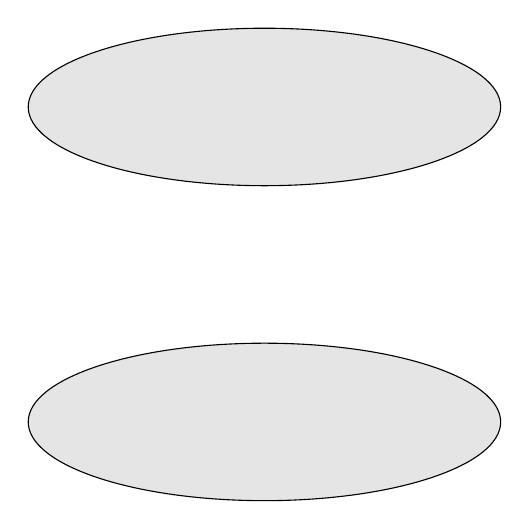
\begin{tikzpicture}
\cylindre[1]{3}{4}
\filldraw[fill=gray!20] (0, 0) ellipse [x radius = 3cm, y radius = 1cm];
\filldraw[fill=gray!20] (0, 4) ellipse [x radius = 3cm, y radius = 1cm];
\tkzDefPoint({3*cos(45)},{1*sin(45)}){M}
\tkzDrawPoint[shape=cross out,scale=2](M)
\tkzDefPoint({-3*cos(45)},{1*sin(45)}){N}
\tkzDrawPoint[shape=cross out,scale=2](N)
\tkzDefPoint({-3*cos(45)},{-1*sin(45)}){P}
\tkzDrawPoint[shape=cross out,scale=2](P)
\tkzDefPoint({3*cos(45)},{-1*sin(45)}){Q}
\tkzDrawPoint[shape=cross out,scale=2](Q)
\tkzDrawSegments[dashed](O',P O',N O',Q O',M)
\tkzDrawSegments[dashed](M,N N,P P,Q Q,M)
\tkzDrawSegments[dotted](M,P N,Q)
\tkzLabelPoint[above right](M){C}
\tkzLabelPoint[above left](N){D}
\tkzLabelPoint[below](P){A}
\tkzLabelPoint[below](Q){B}
\tkzLabelPoint[above](O'){S}





\end{tikzpicture}
\end{exo}
\end{document}